In topic models such as LDA, each abstract ``topic" is characterized by a distribution over words. Such topics are one kind of representation of contexts or scenarios. In this section, we aim to define the topics in Chinese ConceptNet and predict a sentiment value $\in [-1,1]$ on each topic for each concept. Figure~\ref{fig:system1} shows the architecture of our system.

\begin{figure}[!t]
\centering
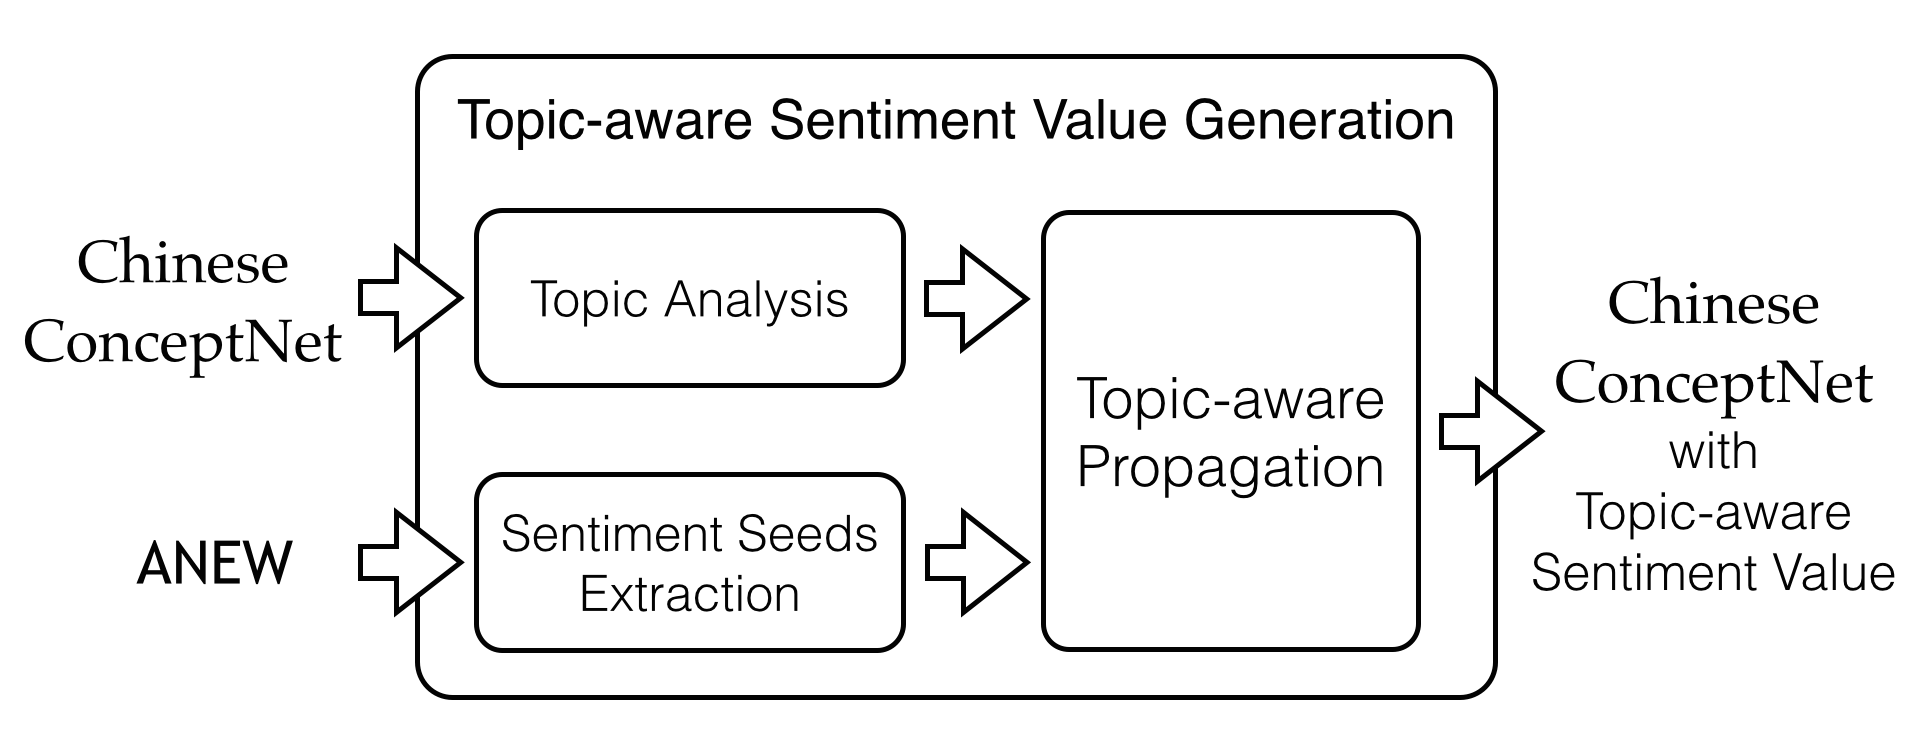
\includegraphics[width=0.5\textwidth]{fig/system1.png}
\caption{System Architecture.}
\label{fig:system1}
\end{figure}

\subsection{Topic Analysis on ConceptNet}
We choose LDA to estimate topics for two reasons: The first one is that LDA allows each document to exhibit multiple topics to different degrees. The second one is that there are corpus parameters after LDA estimation, and we can use these corpus parameters to infer a new document by running the E-step in LDA. 

Similar to the assumption of generating a corpus in LDA, we assume that there is a topic distribution for each concept and its assertions are sampled from this distribution. We aim to find which topic each assertion comes from for each concept. Therefore, we try to apply LDA to find such latent information. 

First, each concept forms a document using its neighbors such that these neighbors have one co-occurrence observation when LDA estimates. See Figure~\ref{fig:noWorkDoc} for illustration, the concept 'do not have to work' generates a document using neighbors as words, with a value indicating how many times the neighbor occurs in assertions.

\begin{figure}[!t]
\centering
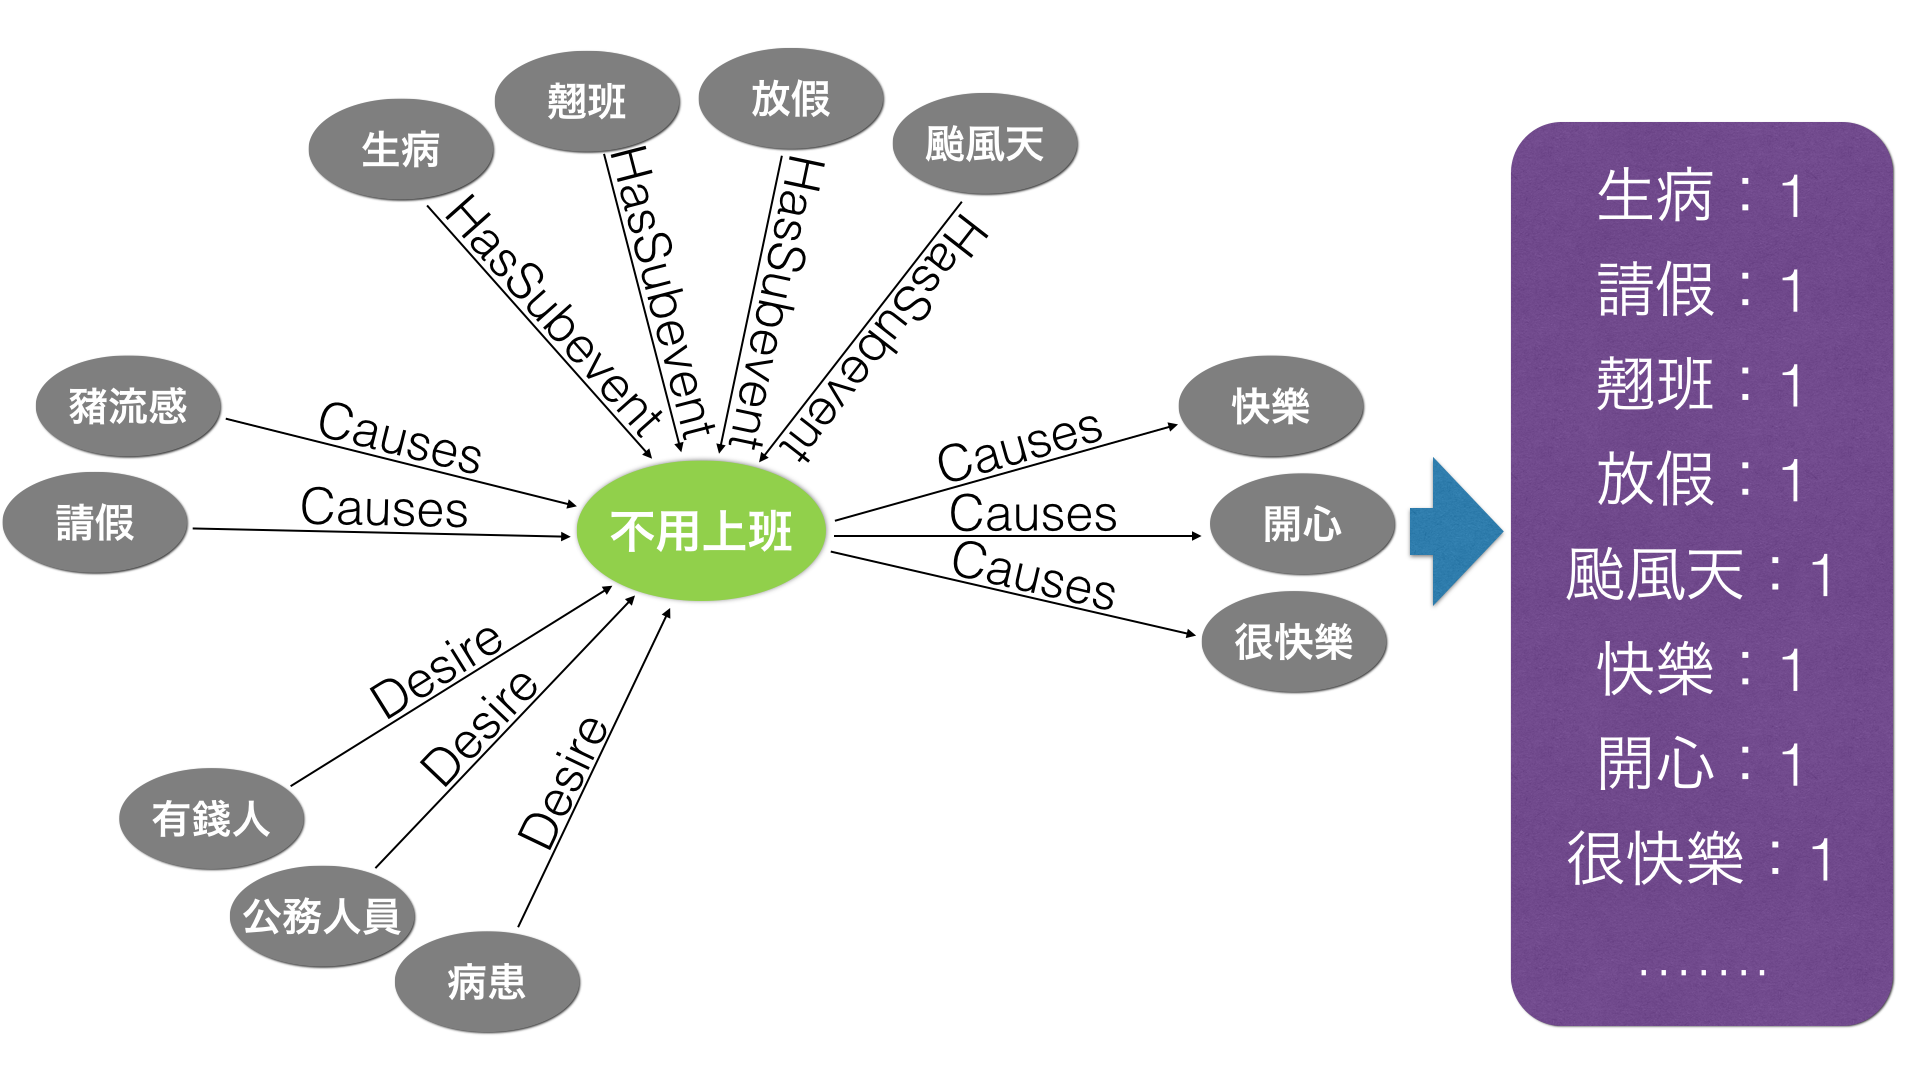
\includegraphics[width=0.5\textwidth]{fig/noWorkDoc.png}
\caption{The document generated by 'do not have to work'.}
\label{fig:noWorkDoc}
\end{figure}

Then we apply LDA to find $\boldsymbol{\theta}_m$ for each document d$_m$ and $z_{m,n}$ for each word $w_{m,n}$ in d$_m$ based on this collection of $M$ documents. Words in each document stand for neighbors of concept, so each resulted $z_{m,n}$ indicates which topicID the neighbor $w_{m,n}$ comes from for concept $c_m$.

As the result, we can design a topic assignment matrix, $\boldsymbol{T}$ where each entry $t_{i,j}$ is $z_{i,j}$ if $j$ is one of $i$'s neighbors, otherwise $unknown$. That is, we can check $t_{i,j}$ for which topicID $i$'s neighbor $j$ belongs to. 

Here we present the result of applying LDA with 10 topics to Chinese ConceptNet. Figure~\ref{fig:wordTop20} shows the per-topic word distribution, $\boldsymbol{\beta}_k$. Each column shows the top 20 words of a topic.

\begin{figure}[!t]
\centering
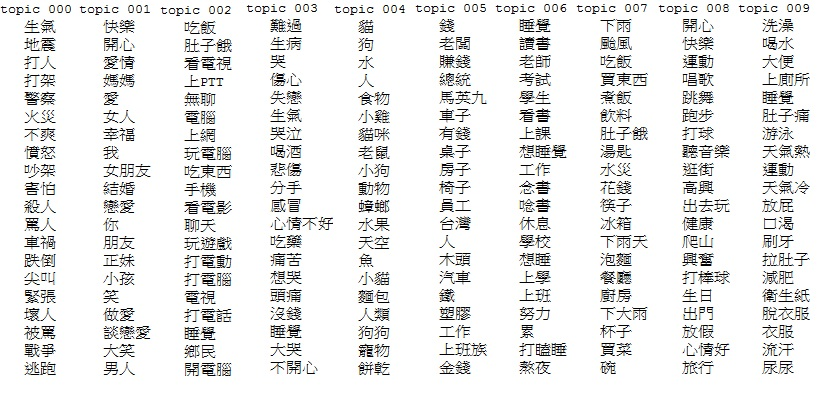
\includegraphics[width=0.5\textwidth]{fig/wordTop20.jpg}
\caption{The top 20 words of each topic.}
\label{fig:wordTop20}
\end{figure}

\subsection{Sentiment Seeds Extraction}
Sentiment seeds here are concepts whose sentiments are known. Common ways to collect sentiment seeds are compiling manually or using other existing sentiment dictionaries. Although concepts we consider here are in Chinese, we use words in Affective Norms for English Words (ANEW)~\cite{Bradley:ANEW99} as our seeds. One reason is its good quality: it was compiled manually by a group of Introductory Psychology class students and provides ratings for 1034 English words through a normative rating procedure. Another reason is that sentiments in ANEW is value-level. Value-level sentiments provide additional intensity information.

We want to assign each concept a sentiment value $\in [-1,1]$ measuring how pleasant or unpleasant people feel about it, so we use the value in ``Pleasure" dimension. Values in ANEW are $\in [1,9]$, so we perform linear normalization on them to value $\in [-1,1]$.

We apply Google Translate to translate all 1034 words in ANEW into Chinese. There may be multiple translations of a English word, we take all of them into account and verify manually. We verify whether the polarities of a English word and its translations are similar. To match more concepts in Chinese ConceptNet, we expand these translations by the approach in our previous research~\cite{Wu:TAAI11}. After expansion, we have 27842 Chinese phrases with sentiment values. In our experiment, there are totally 3047 of them match concepts in Chinese ConceptNet, and then these concepts are used as sentiment seeds.

As the result, given totally $M$ concepts in ConceptNet, we generate a $M \times 1$ vector $\boldsymbol{s}_0$ to denote sentiment values of seed concepts. For each phrase in our expanded translations, if it appears in ConceptNet with concept ID $c$, the ($c$,1) entry of $\boldsymbol{s}_0$ is its linear normalized sentiment value in ANEW. Other entries are $unknown$.

\subsection{Topic-Aware Sentiment Propagation}
After topic analysis, we know which topic each neighbor of each concept comes from by topic assignment matrix $\boldsymbol{T}$. When we predict $c_m$'s sentiment value on the latent topic $z$, we consider neighbors which come from topic $z$ and use their sentiment values on topic $z$. 

However, not all assertions are good for propagation. Next, We select sentiment related relation types and their directions by validation. More specifically, 10\% of positive/neutral/negative sentiment seeds are sampled as validation, and use the remaining 90\% to propagate. The result is shown in TABLE~\ref{table:relRule}.

\begin{table}[]
\centering
\caption{Propagation rules on 13 relation types}
\label{table:relRule}
\begin{tabular}{|l|l|}
\hline
Relation Type    & Propagation rule  \\ \hline
HasFirstSubevent & Not used  		 \\ \hline
MadeOf 			 & Not used  		 \\ \hline
IsA 			 & Not used  		 \\ \hline
AtLocation 		 & Not used  		 \\ \hline
UsedFor 		 & Not used  		 \\ \hline
CapableOf 		 & Not used  		 \\ \hline
MotivatedByGoal  & Latter to Former  \\ \hline
Desires 		 & Not used          \\ \hline
SymbolOf 		 & Former to Latter  \\ \hline
CausesDesire 	 & Not used  		 \\ \hline
Causes 			 & Both Direction    \\ \hline
HasSubevent      & Former to Latter  \\ \hline
PartOf           & Not used  		 \\ \hline
\end{tabular}
\end{table}

Starting from seed concepts, we can use equation~\ref{eq:rndWalk} to iteratively propagate sentiment values on different topics. We design $\boldsymbol{W}$, the $M \times M$ propagation matrix by Algorithm~\ref{alg:wmatrix}. Each element $w_{i,j}$ denotes the weight of sentiment value propagation from concept $j$ to concept $i$.

\begin{algorithm}[htb]
  \caption{determine $\boldsymbol{W}$ for a given topic $z$}
  \label{alg:wmatrix}
  \begin{algorithmic}[1]
  	\Require
  		$z$: current topicID; 
  		$\boldsymbol{T}$: topic assignment matrix;
  		$\text{A} = \{(c1,c2,rel)\}$: all ConceptNet assertions;
    \Ensure
     	$M \times M$ propagation matrix $\boldsymbol{W}$;
	\State initialize $M \times M$ matrix $\boldsymbol{W}$ with each entry $w_{i,j} = 0$    
    \For{each assertion $(c_i,c_j,rel)$ in A}
    \label{code:ruleStart}
    	\State rule = searchPropagationRule($(c_i,c_j,rel)$);
		\If{rule = ``Former to Latter"}
			\State $w_{j,i} \pluseq 1$;
		\ElsIf{rule = ``Latter to Former"}
			\State $w_{i,j} \pluseq 1$;
		\ElsIf{rule = ``Both Direction"}
			\State $w_{j,i} \pluseq 1$, $w_{i,j} \pluseq 1$;
		\EndIf
	\EndFor
	\label{code:ruleEnd}
    
    \For{each $t_{i,j}$ in $\boldsymbol{T}$}
    \label{code:separateContextStart}
		\If{$t_{i,j} \neq z$}
			$w_{i,j} = 0$;
			\Comment{For concept $i$, consider only neighbors in topic $z$}
		\EndIf
    \EndFor
    \label{code:separateContextEnd}
    \State \Return $\boldsymbol{W}$;
  \end{algorithmic}
\end{algorithm}

We can design the propagation matrix for each topic and use it to propagate sentiment values separately. No matter which topic, propagation starts from $\boldsymbol{s}_0$ because the seeds are less ambiguous on different topics. In each iteration $i$, we perform in-link normalization to the propagation matrix. After propagating $iteration$ times, we have the final $\boldsymbol{s}_{iteration}$, which stands for the final sentiment values on topic $z$ for all concepts in ConceptNet. We set sentiment value to $0$ for concepts which are still labelled $unknown$ in $\boldsymbol{s}_{iteration}$. Then, this process repeats for other topics. Finally, each concept has a sentiment value $\in [-1,1]$ on each topic.
